%\title{LaTeX Portrait Poster Template}
%%%%%%%%%%%%%%%%%%%%%%%%%%%%%%%%%%%%%%%%%
% a0poster Portrait Poster
% LaTeX Template
% Version 1.0 (22/06/13)
%
% The a0poster class was created by:
% Gerlinde Kettl and Matthias Weiser (tex@kettl.de)
% 
% This template has been downloaded from:
% http://www.LaTeXTemplates.com
%
% License:
% CC BY-NC-SA 3.0 (http://creativecommons.org/licenses/by-nc-sa/3.0/)
%
%%%%%%%%%%%%%%%%%%%%%%%%%%%%%%%%%%%%%%%%%

%----------------------------------------------------------------------------------------
%	PACKAGES AND OTHER DOCUMENT CONFIGURATIONS
%----------------------------------------------------------------------------------------

\documentclass[a0,portrait]{a0poster}

\usepackage{multicol} % This is so we can have multiple columns of text side-by-side
\columnsep=100pt % This is the amount of white space between the columns in the poster
\columnseprule=3pt % This is the thickness of the black line between the columns in the poster

\usepackage[svgnames]{xcolor} % Specify colors by their 'svgnames', for a full list of all colors available see here: http://www.latextemplates.com/svgnames-colors

\usepackage{times} % Use the times font
%\usepackage{palatino} % Uncomment to use the Palatino font

\usepackage{graphicx} % Required for including images
\graphicspath{{figures/}} % Location of the graphics files
\usepackage{booktabs} % Top and bottom rules for table
\usepackage[font=small,labelfont=bf]{caption} % Required for specifying captions to tables and figures
\usepackage{amsfonts, amsmath, amsthm, amssymb} % For math fonts, symbols and environments
\usepackage{wrapfig} % Allows wrapping text around tables and figures

\begin{document}

%----------------------------------------------------------------------------------------
%	POSTER HEADER 
%----------------------------------------------------------------------------------------

% The header is divided into two boxes:
% The first is 75% wide and houses the title, subtitle, names, university/organization and contact information
% The second is 25% wide and houses a logo for your university/organization or a photo of you
% The widths of these boxes can be easily edited to accommodate your content as you see fit

\begin{minipage}[b]{0.74\linewidth}
    \VeryHuge \color{NavyBlue} \textbf{Status of the ETMC ensemble generation effort} \color{Black}\\ % Title
    % \Huge\textit{Subtitle}\\[2.4cm] % Subtitle
    \Large \textbf{M.~Garofalo$^{a)}$, B.~Kostrzewa$^{b)}$}\\[0.5cm] % Author(s)
    \Large $^{a)}$ Helmholtz-Institut f{\"u}r Strahlen- und Kernphysik (Theorie), University of Bonn, 53115 Bonn, Germany\\
    \Large $^{b)}$ High Performance Computing and Analytics Lab, University of Bonn, 53115 Bonn, Germany\\
    % \Large \texttt{saibi-hakim@mine.kyushu-u.ac.jp} --- +81 (092) 802 3316\\
\end{minipage}
%
\begin{minipage}[b]{0.26\linewidth}
    % \includegraphics[width=7cm]{logo.png}\ 
    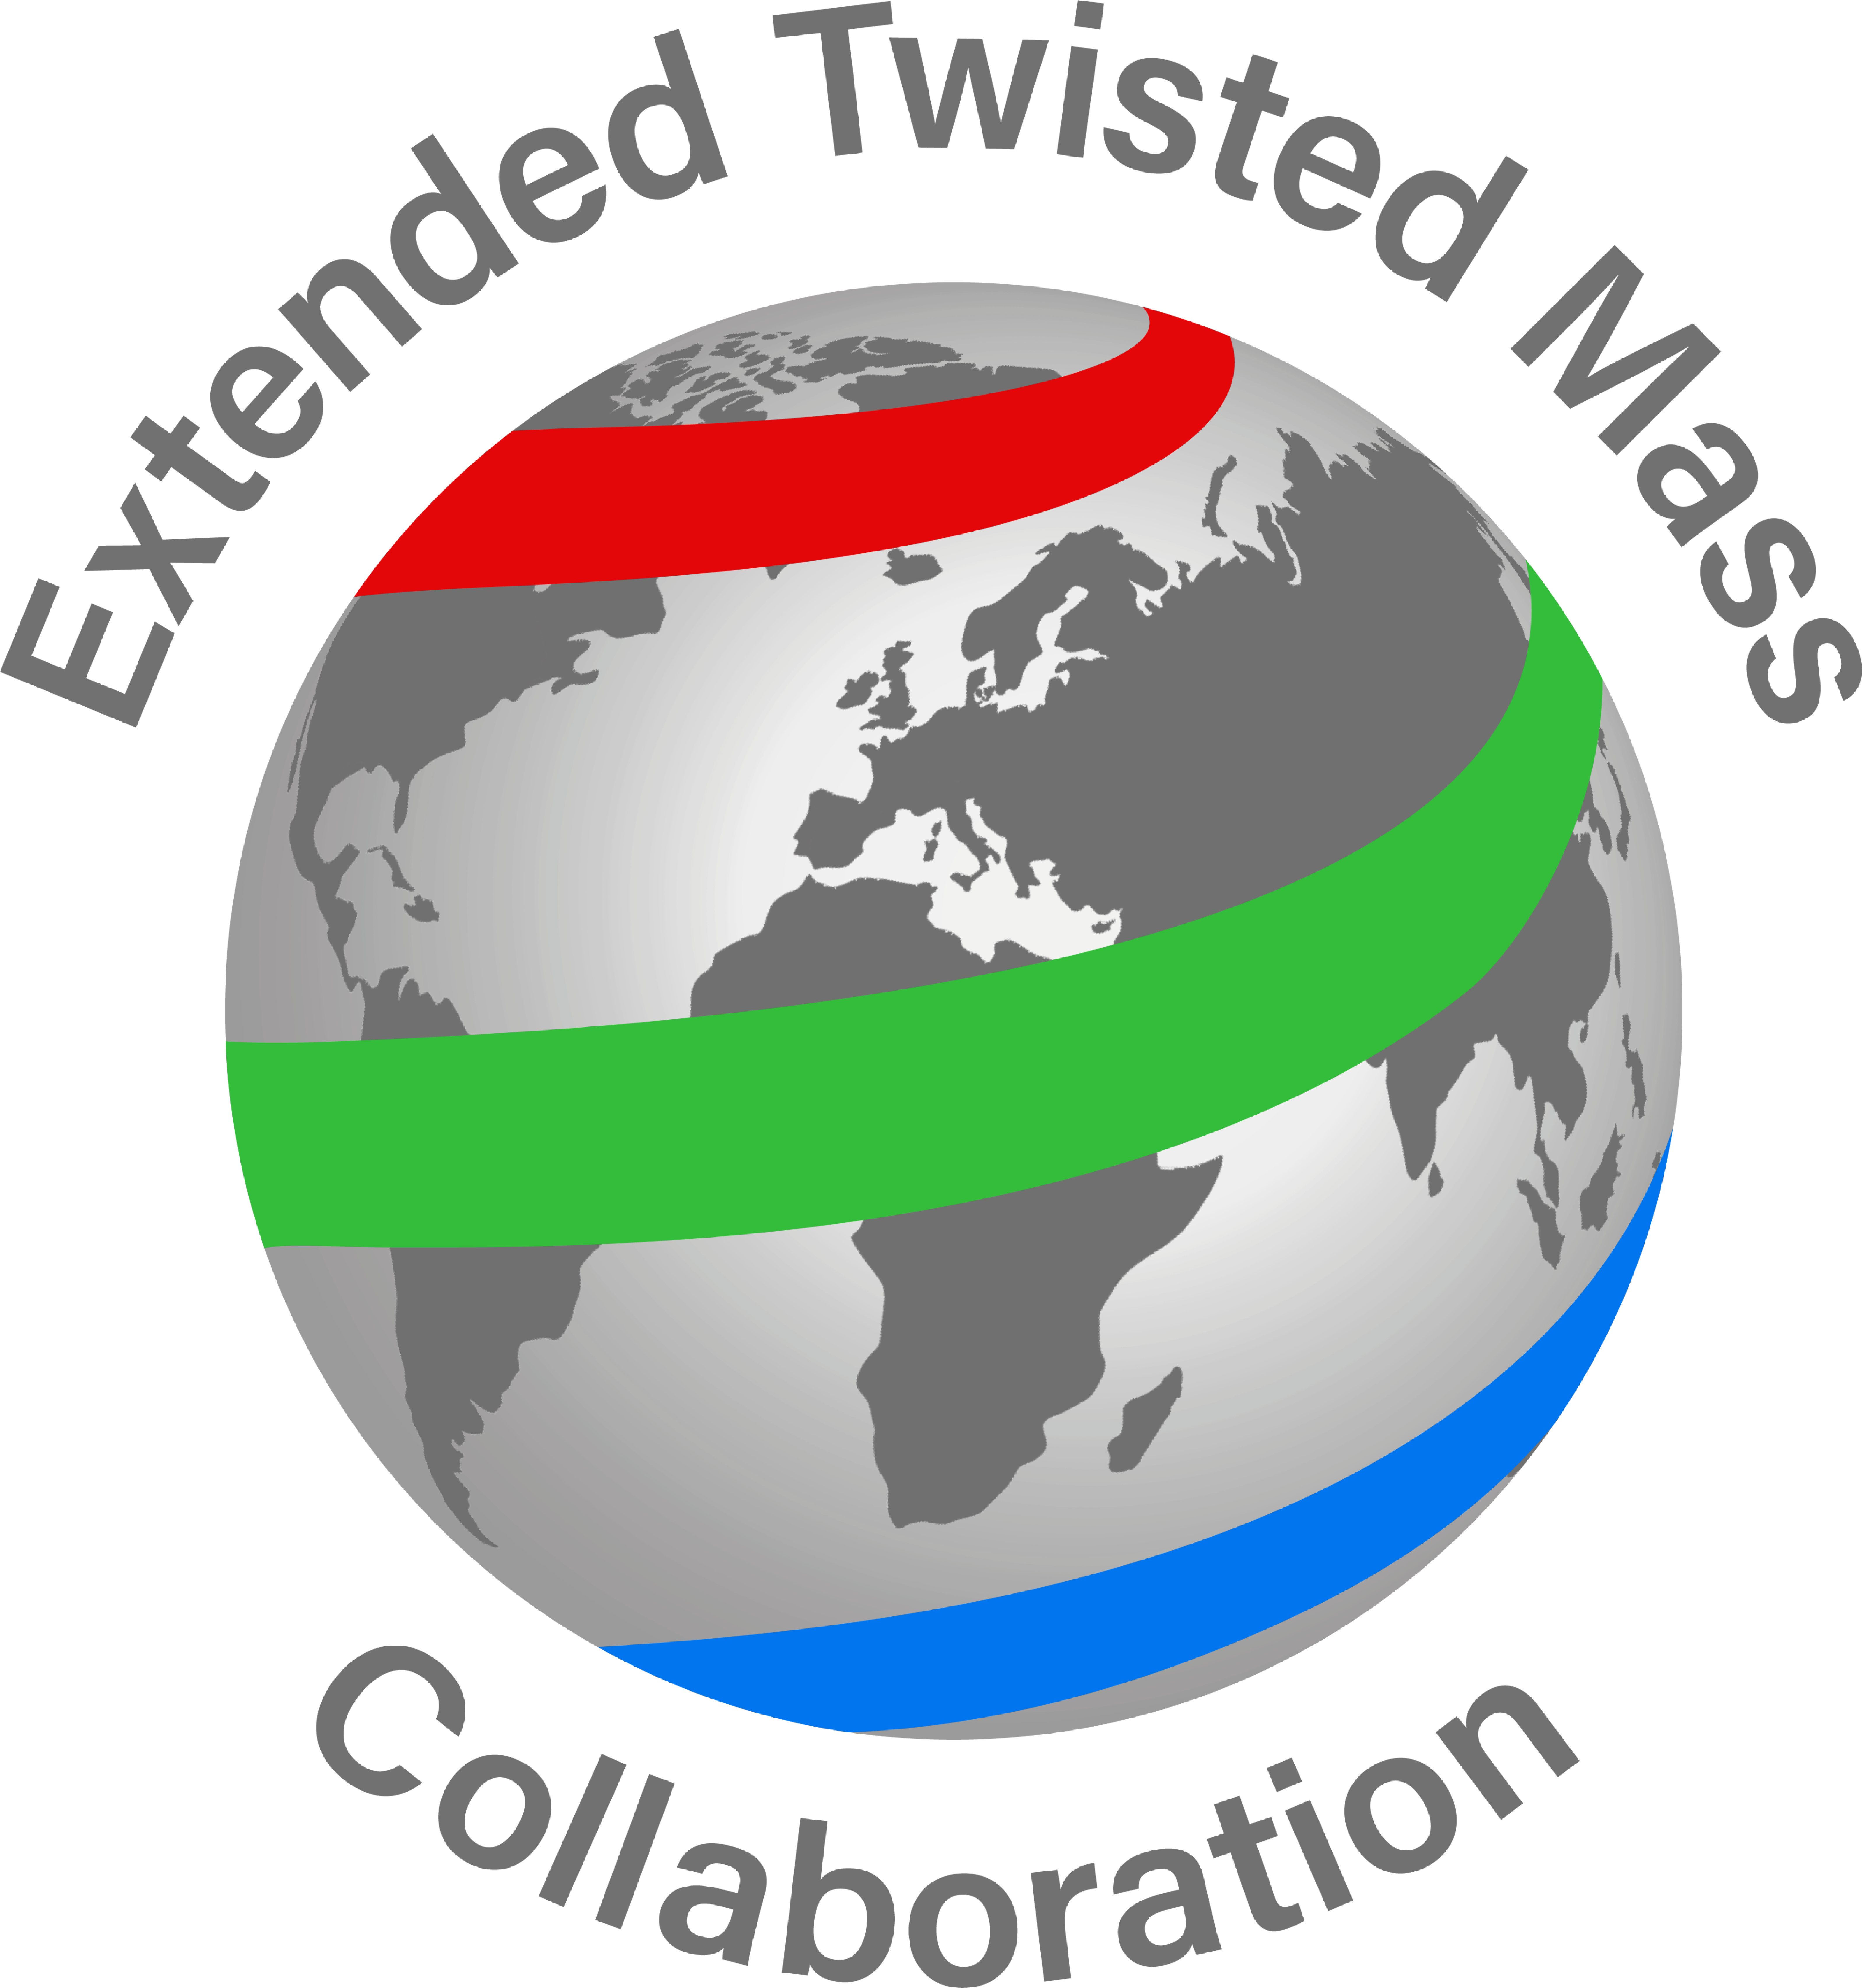
\includegraphics[width=14cm]{figures/Logo_ETMC_RGB.pdf}
\end{minipage}

\vspace{1cm} % A bit of extra whitespace between the header and poster content

%----------------------------------------------------------------------------------------

\begin{multicols}{2} % This is how many columns your poster will be broken into, a portrait poster is generally split into 2 columns

    %----------------------------------------------------------------------------------------
    %	ABSTRACT
    %----------------------------------------------------------------------------------------

    \color{Navy} % Navy color for the abstract

    \begin{abstract}
        The electrical energy from renewables in Algeria contributed about 3.4\% (280 MW) in 2008 of a total power of 8.1 GWe and will reach 5\% by the year 2017 according to the Algerian Electricity and Gas Regulation Commission (CREG). The country’s target is reaching 40\% by 2030. The geothermal resources in Algeria are of low-enthalpy type. Most of these geothermal resources are located in the north of the country and generate a heat discharge of 240 MWt.
    \end{abstract}
    %----------------------------------------------------------------------------------------
    %	INTRODUCTION
    %----------------------------------------------------------------------------------------

    \color{Black} % SaddleBrown color for the introduction
    \section*{Introduction}
    Algeria is situated in northern Africa, bordering the Mediterranean Sea, between Morocco and Tunisia. Algeria has the 9th-largest reserves of natural gas in the world. It ranks 16th in proved oil reserves. Currently, more than 98 \% of Algeria's electricity generation comes from fossil-fuel resources.
    \begin{itemize}
        \item Geothermal exploration program started in 1967 by National Oil Comapny SONATRACH.
        \item From 1983 onwards the geothermal research has been continued by the Renewable Energies Center of Algeria (CDER).
    \end{itemize}

    %----------------------------------------------------------------------------------------
    %	CONCLUSIONS
    %----------------------------------------------------------------------------------------

    \color{SaddleBrown} % SaddleBrown color for the conclusions to make them stand out

    \section*{Conclusions}
    Despite being a petroleum- and gas-rich country, Algeria is making efforts to exploit its renewable energies. The Algerian government has adopted new renewable energy laws and financial support for the investors to facilitate the exploitation of the renewable energies for electricity production and direct utilizations. Algeria has relatively abundant geothermal resources especially in the northeastern parts but not totally used.
    \color{Black} % Set the color back to DarkSlateGray for the rest of the content

    %----------------------------------------------------------------------------------------
    %	FORTHCOMING RESEARCH
    %----------------------------------------------------------------------------------------

    \section*{Forthcoming Research}

    Simulation of thermodynamic properties of the thermal fluid and power output with longevity using geological, hydrogeological, and geothermal data from NE-Algerian geothermal reservoirs.

    %----------------------------------------------------------------------------------------
    %	REFERENCES
    %----------------------------------------------------------------------------------------

    % \nocite{*} % Print all references regardless of whether they were cited in the poster or not
    \bibliographystyle{plain} % Plain referencing style
    \bibliography{sample} % Use the example bibliography file sample.bib

    %----------------------------------------------------------------------------------------

\end{multicols}
\end{document}